\section{Semi-Inclusive DIS}

% 
% This section is a mini version of Nate's thesis.
%

% Background 
% ----------
% Multiplicities are provided by HERMES and COMPASS, JLab has provided moments
% analysis.  There has been no measurement to date of the fully differential 
% cross section for pion SIDIS.  Collaborating with Nate Harrison, we present
% that result here.


% Method 
% ------
% We perform analysis of E1-F charged pions in the kinematic region given 
% by (list the binning).  We perform acceptance corrections based on (model)
% as well as radiative corrections based on (model).  

% Results
% -------
% We find the differential cross section in 5-D space

% Conclusion 
% ----------
% These data can be used as an observable directly sensitve to the 
% the structure function moments cos and cos2 without having the 
% typical ratio of the unpolarized part.  As such, they should prove
% useful in model-dependent studies of TMDs.

Multiplicities for unpolarized pion SIDIS have been provided by HERMES and COMPASS, however no measurement has been made of the absolute cross section.  In this section, a collaborative effort between the author and Nathan Harrison is described that will produce the differential cross section for $\pi^{\pm}$ SIDIS at JLab kinematics.  

Using the E1-F dataset we have identified all events which contain a good electron and a charged pion.  These events are measured fully differentially in 5-D binning of $x$, $Q^2$, $z_h$, $P_{T}^{2}$, and $\phi_h$.  Events are binned in the same way for both $\pi^+$ and $\pi^-$.  Five equal sized bins are chosen in $x$, and each $x$ bin contains 2 bins of $Q^2$ (except for the highest $x$ bin).  The split in $Q^2$ depends on the $x$ value, increasing with increasing $x$ (1.3, 1.7, 2.2, 2.9).  The hadronic variables are binned in a simple manner, with 18 $z_h$ bins between 0-0.9, 20 $P_{T}^{2}$ bins between 0.0 and 1.0 $GeV^2/c^2$.  Finally $\phi_h$ is binned into 36 equal sized bins that span the full 360 degree range. \\

\begin{figure}
  \centering 

  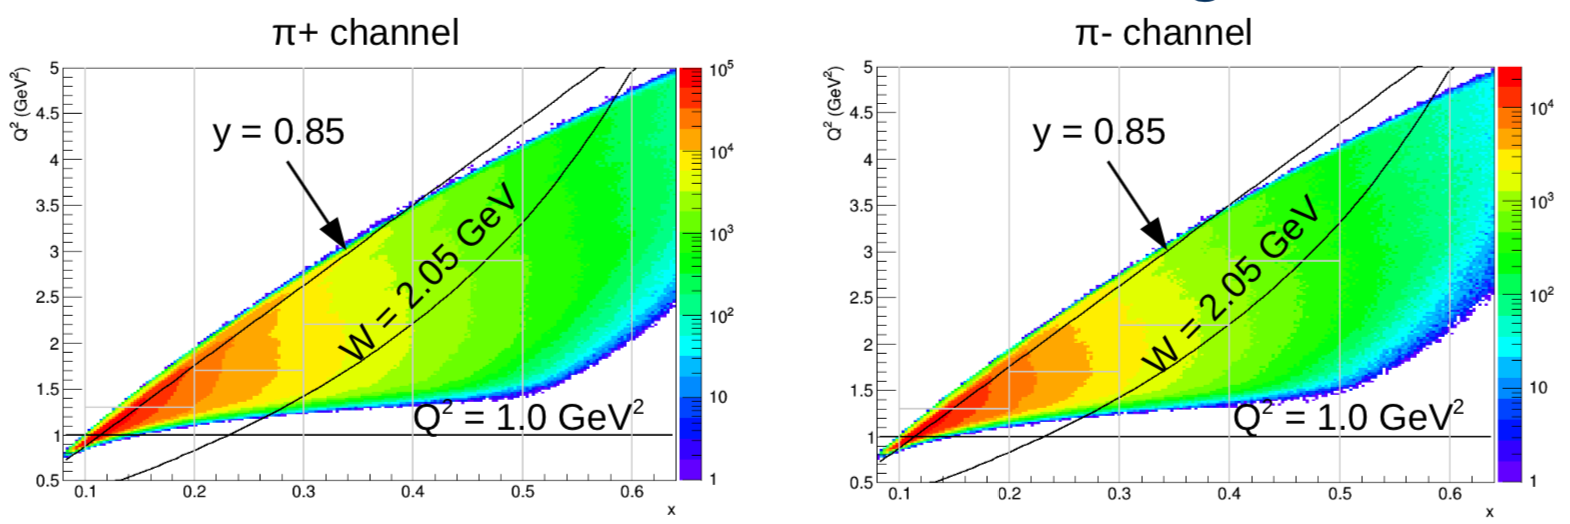
\includegraphics[width=14cm]{image/nathan-xq2.png}
  \caption{Kinematic coverage for $x$ and $Q^2$ shown for both charged pions.  The binning described above for $x$ and $Q^2$ is overlaid in gray.  Figure credit to Nathan Harrison \cite{theses-harrison:2015}.}

\end{figure}

\begin{figure}
  \centering 

  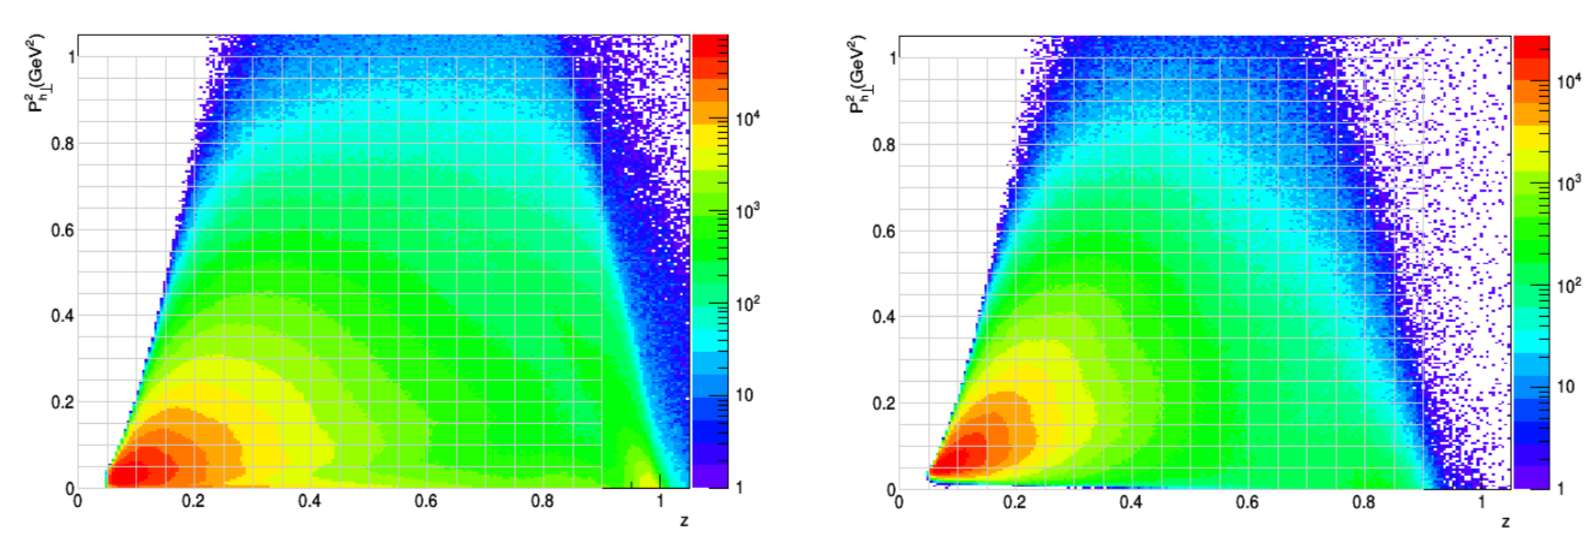
\includegraphics[width=14cm]{image/nathan-zpt.png}
  \caption{Kinematic coverage for $z_h$ and $P_{T}^{2}$ shown for both charged pions (left $\pi^+$ and right $\pi^-$).  Figure credit to Nathan Harrison \cite{theses-harrison:2015}.}

\end{figure}

Acceptance corrections are applied in the same way described in the inclusive section, in this case a Pythia based model is used to generate events.  The kinematic dependence of the reconstructed events matches well with the data, except for the $\phi_h$ axis where an iterative procedure is used to find suitable initial parameters for $A_{UU}^{\cos\phi_h}$ and $A_{UU}^{\cos(2\phi_h)}$.  \\

\begin{figure}
  \centering 

  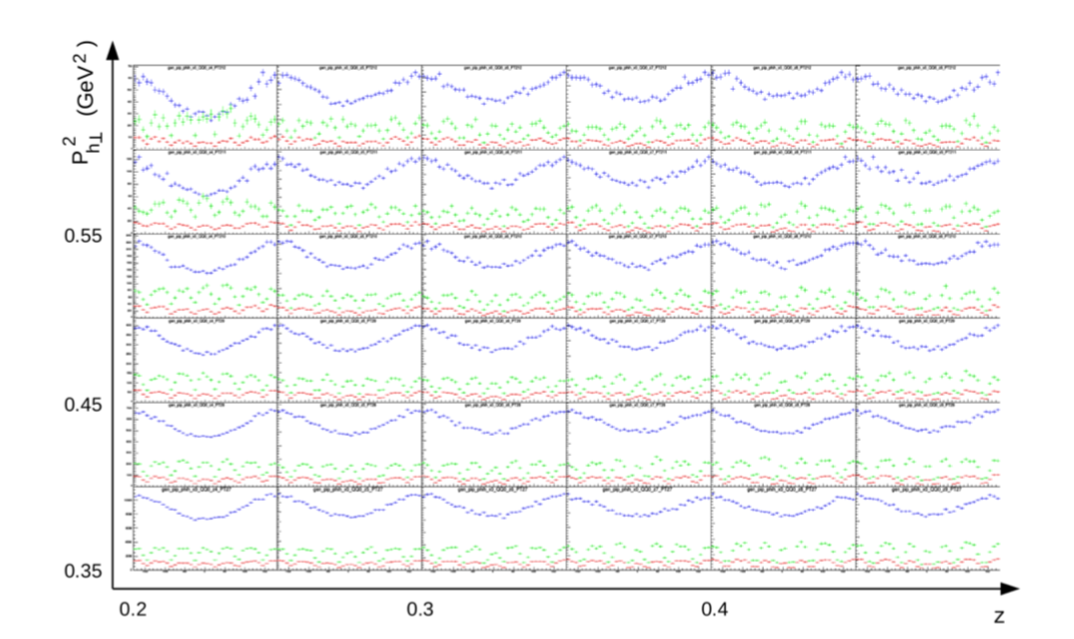
\includegraphics[width=14cm]{image/nathan-acceptance.png}
  \caption{Acceptance for bins of $z_h$, $P_{T}^{2}$ as a function of $\phi_h$ shown in green for $\pi^+$.  Generated events appear here in blue, and reconstructed events in red.  Figure credit to Nathan Harrison \cite{theses-harrison:2015}.}

\end{figure}

Radiative corrections are produced using HAPRAD 2.0, which takes the Born cross section (produced by a model) and produces the radiated cross section.  This procedure is discussed in more detail in the dissertation document.  


\begin{figure}
  \centering 

  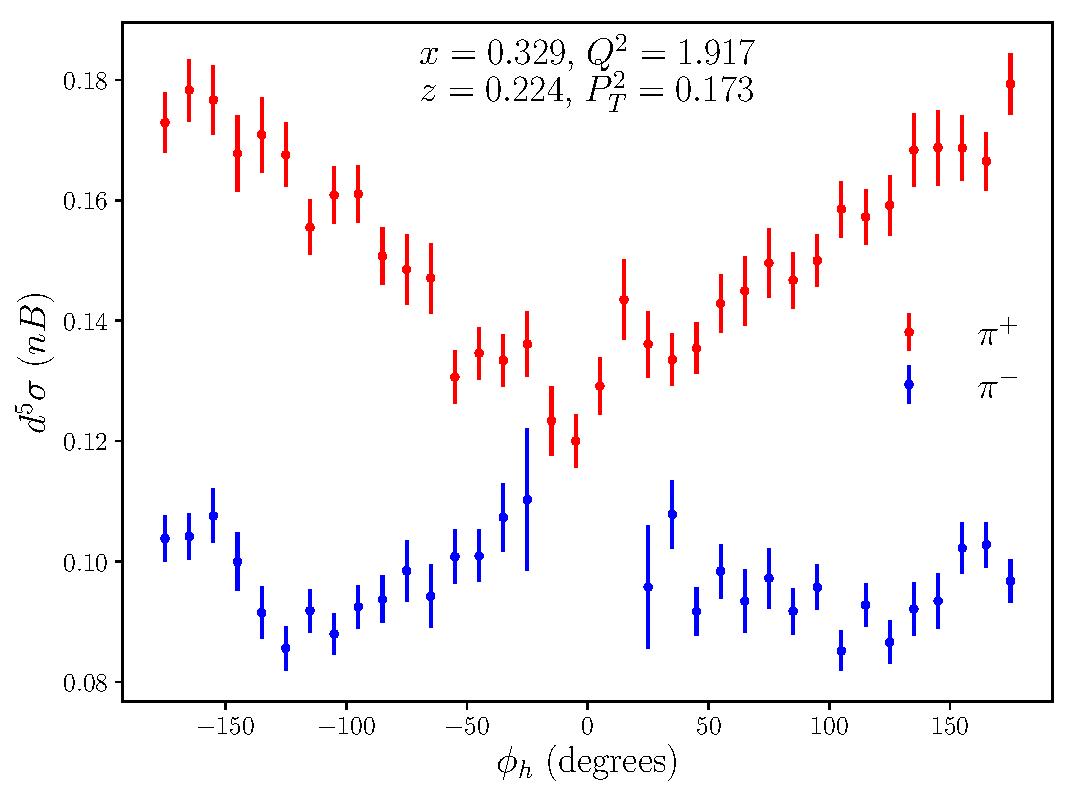
\includegraphics[width=14cm]{image/xs_compare_2043.pdf}
  \caption{The 5-dimensional cross sections are shown for both charged pions, this figure is a preliminary result of our study.  The quoted kinematic point is the center of the bin of measurement.}

\end{figure}
